%!TEX root = ../PhD_thesis__Lilian_Besson

% First chapter begins here
\chapter{Introduction}
\label{chapter:1}

\TODOL{Ecrire les 1.1 et 1.2 en quelques pages}

\abstractStartChapter{}%
%
We start by presenting the context then the problems studied in this thesis.
We further announce the different directions we considered and the solutions we proposed.
We give an overview of our main contributions, alongside a list of publications written in the last three years.
%
The organization of this manuscript is detailed in a flow graph, which highlights that Chapters~\ref{chapter:4} to \ref{chapter:6} are partly independent, but they are all built upon the model and notations introduced on Chapter~\ref{chapter:2}.

\minitocStartChapter{}

% Write miniTOC just after the title
\graphicspath{{2-Chapters/1-Chapter/Images/}}


% ----------------------------------------------------------------------------
\section{Context of this thesis}
\label{sec:1:problems}

% Where
This doctoral thesis started in October $2016$, and finished in October $2019$.
My research took place at the IETR laboratory in Rennes (France), in the SCEE team hosted on the Rennes campus of the engineering college CentraleSupélec.
In Rennes I was supervised by Professor Christophe Moy,
and I was also co-supervised by Doctor Emilie Kaufmann, whom I visited many times at Inria Lille Nord Europe in Lille (France).

% Main problem
At the root of the problems that motivates this thesis are the questions of global warming, and the increase of the world population.
During the last 150 years, mankind has developed a wide range of different communications technology, and since the $1920$s wireless communications between devices have been made possible, and more and more frequent in our lives.
With the avent of Internet of Things networks (IoT), billions of autonomous low-power devices are expected to be deployed world-wide, for a large range of different applications.
It is now well-known that with the current trend of population and with the energy crisis, any newly deployed technology should be cheap and energy efficient,
as well as adapted to serve a large number of people and devices.
%
That is why we are interested in this thesis about the possible applications of embedding a certain kind of Machine Learning algorithms directly into the future IoT devices, in order to improve their battery life and reduce the energy cost of the deployment of IoT networks, by optimizing the wireless communication thanks to embedded decentralized decision making.


\paragraph{From old TV to the IoT standards.}
%
Historically, three families of wireless communication systems have been deployed: first, central broadcasting (\eg, old TV), then centralized bi-directional systems (\eg, 4G or WiFi), and nowadays decentralized broadcasting for the Internet of Things networks (IoT).

% Central broadcasting
Starting from FM radio music and news, then old black-and-white TV and color TV, the first systems were purely made for centralized broadcasting of information. In a large area, one antenna well located emits continuously in a fixed Radio Frequency (RF) band, and many devices can listen to this RF traffic and decode it, for instance to listen to music.
Different standards have been developed, and some of them are still in use today, and their nature requires a central authority that allocates RF bands to different usages (\eg, TV channels etc).
For example, in the city of Cesson-Sévigné where the campus of CentraleSupélec is located, a high RF tower emits on many standards, and in particular the \SI{92.3}{\mega\hertz} band is allocated to a French classical music radio (\emph{Radio Classique}).
Broadcast-based systems are not only used for TV or radio,
and for instance two other famous and world-wide deployed examples are the Global Positioning System (GPS) and infrared remote controllers.

% Two ways communications
However, this kind of mono-directional wireless communications were soon found to not be satisfactory for many applications, and thus bi-directional standards were defined from the $1940$s.
First developed by and for the military, such applications have reached general public usage since the $1970$s.
The greatest achievement of this long-running R\&D domain was the avent of mobile telephony in the $1990$s, which has continued to be more and more present in people lives in the richer countries in the world, with the booming of cellphones since the $2000$s and smartphones since the $2010$s.
In most systems, there is still an antenna in charge of a large area (or cell), and many devices are able to receive and transmit data to the antenna.
Nowadays, the most well-known systems include WiFi, and systems deployed for mobile phone communications, with a long list of standards from 1G, 2G, 3G, 4G and now 5G, still in development in $2019$.
Even if both systems initially differed in usage, as 1G was designed to exchange only voice, and WiFi to link wireless devices at home to an Internet-connected box, they are conceptually very close.
As the systems are cellular, any device knows the antenna (or base station) it is associated with, and the bi-directional nature of their exchanges makes a centralized control possible.
In order to optimize the efficiency of the network, the base station is equipped with decision making algorithms that affects the devices in the cell to the available resources (time slots, RF bands, power etc).
To be able to communicate with the base station without interfering with each others, such affectation should be orthogonal, and led to systems based on Time Division Multiple Access (TDMA) and Frequency Division Multiple Access (FDMA), or more recently to Non-Orthogonal techniques (NOMA).
Traditionally, the base station aimed only at maximizing the Quality of Service (QoS), that englobes the data rate, latency, availability and other measures of performance of the wireless communications to and from the devices.
More recently, green radio has emerged as a solution to the tradeoff between maximizing QoS while minimizing the power consumption of base stations and devices.

% The opposite: decentralized broadcasting, and the age of IoT
Finally, a third kind of systems are of the opposite kind, and can be designed as decentralized broadcasting: an antenna is still in charge of many devices, but such devices can only send up-link packets, and the only down-link data they can receive are short acknowledgements sent from the base-station to indicate success or failure of an up-link packet.
This family of wireless systems are referred to as Internet of Things,
and a typical example of application is for sensor networks.

For the future development of smart grids, smart cities, smart homes, or smart agriculture, sensor networks are promised to be widely deployed.
Two examples of future applications that are already in deployment, in France or other countries, are connected buildings and connected agriculture.
For buildings, the main goal is to reduce the cost of heating empty buildings and use temperature sensor networks to get accurate and regular data about the temperature in each room and each floor, and let the centralized heat control optimize its cost and energy consumption.
For agriculture, one example can be to equipped every cow (in large farms) with a sensors that emits biological information, such as body temperature or stress level etc, in order to optimize the time of milking and monitors the health of the animals.

This third kind of wireless systems are characterized by their decentralized nature: due to the really limited information that the base station can send to the devices, it is no longer possible to optimize the efficiency of the network from the centralized point-of-view of the base station.
In the present and future IoT networks, many devices of heterogenous nature are using the same antenna for many different applications.
A common hypothesis is that such IoT devices have a strong constraint on their power consumption, as most of them will be deployed without a direct power access and will use a battery, which duration should be maximized (typically more than 10 years).
Another common constraint for IoT devices is their low duty cycle, as most applications target one to a few messages sent by day, in strike opposition to the high data-rate pursued for centralized systems such as 4G/5G and WiFi.
%
In this thesis, we study Internet of Things networks, and these two constraints of low power consumption (or long battery life) and low duty cycle are essential.


\paragraph{Cognitive Radio.}
%


\begin{itemize}
    \item
    Joseph Mittola \cite{Mitola99}:
    \emph{``A really smart radio that would be self-, RF- and user-aware, and that would include software technology and machine learning capabilities along with a lot of high-fidelity knowledge of the radio environment.}

    \item
    Simon Haykin \cite{Haykin05}:
    \emph{``A CR is an intelligent wireless communication system that is capable of being aware of its surroundings, learning, and adapting its operating parameters (\eg, transmit power and carrier frequency) on the fly with an objective of providing reliable anytime, anywhere, and spectrally efficient communication.}
\end{itemize}


\newpage

But de ce chapitre :
le lecteur va savoir en quelques pages

- contexte historique technologique => okay

- les télécoms ? télécoms décentralisées ? => okay

- l'IoT c'est quoi ? exemple d'applications ? => okay ?

- les bandits c'est quoi ?

- les bandits multi-joueurs décentralisés, pourquoi ?

- pourquoi étudier ça ?

- OK qu'est ce qu'on a proposé et pourquoi ? => plan des contributions, bullet point (1ère version, je pourrai faire mieux après)

- OK comment lire la thèse => le plan Figure~\ref{fig:1:organization}


\TODOL{Je dois faire ça d'ici mercredi matin}
% Je peux m'inspirer beaucoup de la thèse de Navik...
% https://tel.archives-ouvertes.fr/tel-01668536/document

OK commencer par un paragraphe qui explique qu'on étudie les télécom dans le but de les rendre automatiquement plus efficace, plus verte, plus adaptative

OK commencer par décrire ce sur quoi porte la thèse, en deux phrases qui réduisent le cadre

- technologies de l'information > télécommunications > communications sans fil > radio intelligente > DSA > OSA
- apprentissage statistique (machine learning) > séquentiel > par renforcement > information partielle (bandits)

Je peux piquer les quelques figures chouettes de Navik (en attendant la version finale ou je referai mes figures)

Il faut expliquer ce que c'est que la radio intelligente, et le cas de l'OSA

je peux faire comme Navik, donner des définitions de la CR, citant d'autres travaux

Il faut expliquer ce que c'est que les bandits, rapidement, et leur application à l'OSA

expliquer ce que Christophe Moy, Wassim Jouini, Navik Modi etc ont fait depuis 2009


quels nouveaux challenges en 2016 ?

autre direction

- radio intelligente > internet des objets


directions de recherches

- réfléchir aux modèles, quelles hypothèses sont retirées comparé au modèle OSA

- analyser mathématiquement les modèles

- proposer des solutions : algorithmes, dont la convergence est justifiée, ou heuristiques

- des simulations logicielles

- des démonstrations matérielles

- et en bonus on obtient aussi de belles contributions théoriques

\newpage

\subsection{Reinforcement learning}

\tikzstyle{block} = [align=center, draw, fill=gray!25, rectangle, minimum height=3em, minimum width=6em]
\begin{figure}[h!]
    \centering
    \resizebox{0.40\textwidth}{!}{
        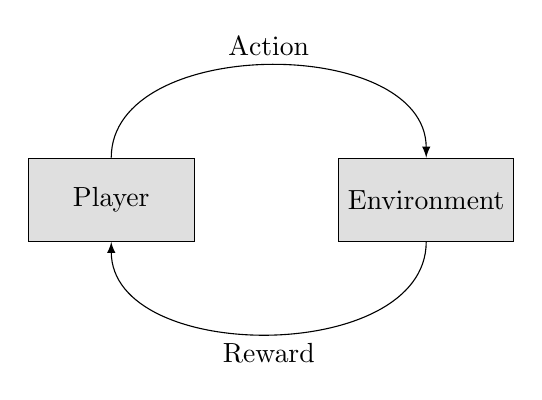
\begin{tikzpicture}[auto,node distance=5cm,>=latex,scale=2]
            %
            % We start by placing the blocks
            \node [block] (player) at (0,0) {Player};
            % We draw an edge between the player and system block to
            \node [block] (environment) at (2,0) {Environment};
            % Once the nodes are placed, connecting them is easy.
            \draw [->] (player) to[bend left=90] node[pos=0.5] {Action} (environment);
            \draw [->] (environment) to[bend left=90] node[pos=0.5] {Reward} (player);
            %
        \end{tikzpicture}
    }
\caption{Reinforcement learning cycle.}
\label{fig:1:ReinforcementLearningCycle}
\end{figure}

\hline{}
\newpage


\paragraph{On Cognitive Radio.}

Des thèses précédentes avaient déjà identifié l'apprentissage séquentiel comme étant pertinent pour la radio intelligente.
On peut citer les travaux de \cite{Jouini09,Jouini10,Jouini12}, qui ont notamment souligné les points suivants :

\begin{itemize}
    \item implémentation peu couteuse en ressources d'exécution (temps et mémoire), contrairement aux autres approches de décision basées sur l'optimisation, ou d'autres techniques d'IA,
    \item capacité à apprendre depuis zéro (pas de phase de pré apprentissage durant laquelle le système ne fait rien d'autre qu'apprendre), et forte capacité à s'adapter automatiquement à un nouveau contexte,
    \item coordination décentralisée possible de plusieurs joueurs, sans qu'il n'y ait de communication autorisée entre eux,
    \item approche cohérente dans un système décentralisé, si chaque objet sans fil apprend de son côté plutôt que de recevoir des instructions d'une station de base,
    \item résistent aux erreurs d'apprentissage
\end{itemize}

Ces techniques ont aussi permis d'identifier les bandits multi-bras comme le bon modèle d'apprentissage séquentiel statistique dans le contexte de la radio intelligente.
Des algorithmes de MAB ont été utilisés avec succès dans différents contextes :

\begin{itemize}
    \item le choix de la configuration radio, avec par exemple \cite{KerkoucheAlami18} récemment,
    \item l'accès dynamique au spectre, et en particulier l'accès opportuniste (OSA) \cite{Jouini09}.
\end{itemize}

Mais le cas OSA a plusieurs faiblesses :

\begin{itemize}
    \item il est trop futuriste, car la régulation des fréquences ne permet pas encore (et en est très loin) de l'appliquer en situation réelle,
    \item en l'absence de régulation coordonnée, chaque cas d'OSA dépendra de la bande considérée (et comment les objets "licencees" s'y comportent), mais les études de l'équipe SCEE ont montrées que les approches MAB sont capables de s'adapter à tous les cas,
    \item le retour de décision utilisé dans l'OSA repose sur le sensing, qui est le maillon faible de la boucle (pas encore assez fiable pour être utilisé en vrai).
    \item d'où l'idée d'utiliser les MAB en Cognitive Radio, dans les bandes non licenciées, dès 2011 \cite{Jouini12}. Dans ce cas, le contexte est comme en OSA, mais sans PU, et pas de sensing.
\end{itemize}

Pour toutes ces raisons, le cadre de l'internet des objets (IoT) apparaît comme idéal car c'est un cadre qui s'affranchit des contraintes de l'OSA.

Par conséquent, cette thèse vise à refermer certaines portes qui étaient encore intéressantes à étudier dans la suite de ce qui a été considéré pour l'OSA

\paragraph{On Multi-Armed Bandit.}


% ----------------------------------------------------------------------------
\section{Considered problems}
\label{sec:1:problems}

\TODOL{Write this!}

\subsection{Spectrum scarcity}


\subsection{Low-consumption IoT devices for the future}


% ----------------------------------------------------------------------------
\section{Considered solutions}
\label{sec:1:solutions}

\TODOL{Write this!}


\subsection{Online/sequential machine learning to automatically improve wireless communications on the run}

\subsection{Example: Opportunistic Spectrum Access (OSA) in licensed bands}


\paragraph{Applications for Opportunistic Spectrum Access.}
% Detail the previous work from our team SCEE on bandits + OSA : Wassim, Navik

\TODOL{Tous les paragraphes suivants sont copiés collés de plus tard dans la thèse, je peux les réadapter ici, et les supprimer/raccourcir plus loin}

The focus of this work is on cognitive radio and IoT networks, where arms can represent wireless orthogonal channels, but more generally any resource characterizing the communication between a wireless device and a gateway (\eg, spreading factor for LoRa \cite{KerkoucheAlami18}, power allocation for NOMA etc). In cognitive radio using centralized supervision, for instance if the gateway can decide the allocation of devices to resources, MAB can also be used to let the gateway explore different allocations and learn by itself a good allocation, see for instance this article that consider 5G-like networks with small cells \cite{Maghsudi16}.

Previous works of our SCEE team showed that MAB can be used to model the problem of spectrum access for a secondary user accessing a licensed spectrum.
In this model, arms represent a finite set of orthogonal channels, \ie, different frequency bands in a licensed spectrum.
In the model with sensing, the samples $Y_{k,t}$ represents the feedback obtained by the CR-equipped device after sensing the channel $k$ at time $t$.
A reward of $r(t) = 1$ indicates that no Primary User was sensed, while a reward of $r(t)=0$ indicates that the channel $k$ is busy at time $t$ and no uplink message can be sent.
%
This model was first introduced by Wassim Jouini during his PhD thesis,
in \cite{Jouini09} and later studied in both \cite{Jouini10,Jouini12}.
Proof-of-concepts using real-world radio hardware was first propsed in \cite{MoyWSR2014,RobertSDR2014}.

\TODOL{Je sais pas à quel point je veux parler de la thèse de Navik? Peut-être que j'en aurai dit assez au Chapitre 1, et que là ça suffira..}
In a second PhD thesis supervised by Christophe Moy \cite{Modi17PhD}, Navikkumar Modi studied the impact
of using MAB algorithms to optimize channel selection
on the battery life of a wireless device.
On the one hand, running a MAB algorithm such as UCB-like algorithms was proven to be useful and can bring significant improvement in terms of successful transmission rates, directly increasing the battery life of the device.
On the other hand, classical MAB algorithms tend to switch arms a lot of times, especially in the beginning of the learning process, and this induces a lot of dynamical hardware reconfiguration for the wireless device, as selecting a different channel requires a change in the radio hardware used by the device.
Each hardware reconfiguration costs energy for the device, and quickly switching algorithms will lead to a reduction of the battery life.
The tradeoff between the two aspects is studied empirically in
\cite{modiDemo2016}.
%
Another interesting works is \cite{Modi17QoS}.


We already explained in Chapter~\ref{chapter:1} that
unlicensed bands are more and more used and considered for mobile and LAN communication standards (WiFi, LTE-U), and for Internet of Things (IoT) standards for short-range (ZigBee, Z-Wave, Bluetooth) and long-range (LoRaWAN, SIGFOX, Ingenu, Weightless) communications \cite{Centenaro16}.
This heavy use of unlicensed bands, in particular with the expected exponential growth of the number of IoT devices, will cause performance drop, due to radio collisions that could even compromise IoT promises.

Efficient Medium Access (MAC) policies allow devices to avoid interfering traffic and can significantly reduce the spectrum contention problem in unlicensed bands.
As end-devices battery life is a key constraint of IoT networks,
and as IoT networks are decentralized (\ie, the devices initiate transmissions),
this leads to IoT protocols using as low signaling overhead as possible and simple ALOHA-based mechanisms.
%
In this chapter, we analyze the performance of Multi-Armed Bandits (MAB) algorithms, that could be used in combination with a time-frequency slotted ALOHA-based protocol.
Even without changing anything of the level of IoT standards, our proposal is just an add-on capability that can be used on a unit-per-unit basis.
We consider the Upper-Confidence Bound (\UCB) \cite{Auer02}, and the Thompson-Sampling (TS) algorithms \cite{Thompson33,AgrawalGoyal11,
Kaufmann12Thompson}, for the first model. For the demonstration as well as for the second model, without loss of generality, we preferred to focus on heuristics based on the simplest algorithm (\ie, \UCB), to give a clear presentation of the different ideas explored to solve the problem of learning in order to retransmit efficiently.

As detailed in Chapter~\ref{chapter:1},
MAB learning has already been proposed in Cognitive Radio (CR) \cite{Mitola99,Haykin05}, and in particular, for sensing-based Dynamic Spectrum Access (DSA) in licensed bands \cite{Jouini10}.
For example,
proof-of-concepts like \cite{kumar2016two} have proven the capability of such approaches on real radio signals for OSA,
and \cite{Maghsudi16} shows how MAB learning can be applied for small cell management in licensed 5G networks.
Some analysis on real radio measurements made for HF ionospheric channels have also proven that solutions based on MAB learning is appropriate and solves efficiently this kind of decision-making problems on real-world wireless signals \cite{Melian15}.
Recent works show that stationary MAB algorithms work well to solve reinforcement learning models that represent accurately real-world radio problems.
Recently, TS and \UCB{} algorithms have been used for improving the spectrum access in (unlicensed) WiFi networks, for instance by \cite{Toldov16} or \cite{Wilhelmi19collaborative,Wilhelmi19potential}.
% However, even with only one dynamic user using the learning algorithm, the background traffic or the traffic of the other devices is never really stationary or \iid{}.

We present in Section~\ref{sec:4:firstModel} how the MAB algorithms can be used in a unlicensed but frequency- and time-slotted IoT network.
Several devices are using bandit algorithms, and the assumptions made by the stochastic bandit algorithms are not satisfied: as several agents learn simultaneously and their activation processes are random, their behavior is not stationary.
As far as we know, we provide the first practical study to confirm robustness of the use of stochastic bandit algorithms for decision making in IoT networks with a large number of intelligent devices in the network, which makes the environment ``highly not stationary''.
This specific context makes it very hard to give mathematical proofs of  convergence and efficiency for bandit algorithms (that is why we relax the hypothesis and only consider up-to $M \leq K$ players in Chapter~\ref{chapter:5}).
We then validate the model with a hardware implementation on real radio signals, detailed in Section~\ref{sec:4:gnuradio}.
%
We conclude this chapter by presenting in Section~\ref{sec:4:retransmissions} an extension of this model to take into account another aspect of the ALOHA protocol, that is the possibility for dynamic devices to retransmit their packet if the \emph{Ack} was not received.

As explained before in Chapter~\ref{chapter:1}, the future IoT networks will require to support more and more communicating devices.
In this section, we show that intelligent devices in unlicensed bands can use MAB learning algorithms to improve spectral resource exploitation.
%
We evaluate the performance of two classical MAB learning algorithms, \UCB{} and Thomson Sampling, to handle the decentralized decision-making of Spectrum Access, applied to IoT networks.
We mean by \emph{decentralized} that learning is performed on the device side, and is spread on the totality of the devices in a network.
We also evaluate the learning performance when the number of intelligent end-devices grows.
%
We show that using learning algorithms
firstly extends devices battery autonomy (by reducing the packet-loss-ratio or equivalently, by improving the successful-communication rate),
and secondly does help to fit more devices in such networks, even when all end-devices are intelligent and are dynamically switching from channel to channel.
In the studied settings,
Stochastic MAB learning
% provides an up to $16\%$ gain in terms of successful transmission probabilities, and
has near optimal performance even in non-stationary settings with a majority of intelligent devices.


The aim of this section is to assess the potential gain of learning algorithms in IoT scenarios, even when the number of intelligent devices in the network increases,
and the network usage is more and more fluctuating.
% and the stochastic hypothesis is more and more violated.
To do that, we suppose an IoT network made of two types of devices: \emph{static devices} that use only one channel (fixed in time), and \emph{dynamic devices} that can choose the channel for each of their transmissions. Static devices form an interfering traffic, which could be generated by devices using other standards as well.
Note that instead of assuming that each static device uses a fixed channel, we could also assume a looser hypothesis: if each static device uses a fixed sub-set of the $K$ channels, and a purely uniform random access in its set of considered channels, then \emph{in average} the observed occupancy of the $K$ channels can be modeled as if it were occupied by (more) static devices using only one channel. So our first hypothesis is actually not constraining.
We first evaluate the probability of collision if dynamic devices randomly select channels (that is, a naive approach), and if a centralized controller would optimally distribute all of them in the channels at the beginning of the scenario.
This second approach is ideal, but not realistic the most common situation of decentralized co-located IoT networks, and it is just used here as a reference.
Then, these three reference scenarios allow to evaluate the performance of bandit algorithms, such as \UCB{} and TS, in a decentralized network, in terms of successful communication rate, as it reflects the network efficiency.
We show that these algorithms have near-optimal performance, even when the proportion of end-devices increases and the interfering traffic from other devices becomes less and less stochastic.


\subsection{Example: decentralized learning in unlicensed bands with selfish or orthogonalization-based MAB algorithms}


We evoke here some previous works that similarly implemented proof-of-concepts to show that reinforcement learning algorithms can be used within real-world wireless communications.
Starting from $2010$, the works of Wassim Jouini \cite{Jouini09,Jouini10,Jouini12} were the first ones to propose to use Reinforcement Learning for Cognitive Radio, especially MAB and the \UCB{} algorithm, and from $2014$, proof-of-concepts were developed by Christophe Moy and his student Clément Robert \cite{RobertSDR2014,MoyWSR2014}.
In $2015$ and $2016$, Christophe Moy continued to work on this direction, with a PhD student (Navikkumar Modi) and post-doc (Sumit J. Darak) in our team SCEE, for the following publications
\cite{darak2016bayesian,Darak16,modiDemo2016,kumar2016two}.
Since $2017$, Sumit J. Darak and his team at IIIT Delhi have been very active in the research on cognitive radio using multi-armed bandits, and some of their recent works are illustrated with real-world demo using USRP and the MATLAB/Simulink system
\cite{KumarYadav2018,SawantKumar2018,JoshiKumar2018}.


\TODOL{Je suis content de la suite de l'intro : aperçu des contributions, plans de thèse, liste des publications}

\newpage % WARNING
% FIXME c'est bon tout ce qu'on a avant ?

% ----------------------------------------------------------------------------
\section{Overview of the contributions}
\label{sec:1:contributions}

We can list the following points to summarize the main contributions of this thesis:

\begin{itemize}
    % \item
    % We present the concepts and the notations of the multi-armed bandit problem in Chapter~\ref{chapter:2}, from a mathematical point-of-view.
    % But we also follow a didactic approach as we use an online interactive demonstration designed to let anyone play against a small bandit problem from his/her browser, in Section~\ref{par:2:interactiveDemoDiscoverMAB}.

    % \item
    % We give a short literature review of stochastic bandit algorithms in Section~\ref{sec:2:famousMABalgorithms}.

    \item
    We wrote the most exhaustive open-source simulation library for MAB problems, called SMPyBandits, which is published online under an open-source licence \cite{SMPyBandits,SMPyBanditsJMLR}.
    We present in details its architecture and its features in Chapter~\ref{chapter:3}, along with different examples of its usage.
    A full documentation is available online, as well as exhaustive instructions to reproduce the experiments used in the rest of this thesis.

    \item
    % We present the problem of choosing which algorithm a practitioner should use, or algorithm selection from the rich collection of different MAB available, in Section~\ref{sec:2:chooseYourPreferredBanditAlgorithm}.
    We present in Chapter~\ref{chapter:25} an algorithm called \Aggr{} for aggregation of algorithms as an online solution to the algorithm selection problem, and numerical simulations to illustrate that it achieves state-of-the-art empirical performances
    \cite{Besson2018WCNC}.
    % with \textbf{Aggregator} (WCNC 2018)

    \item
    We propose different models for IoT networks, in Chapter~\ref{chapter:4}, where end-devices with cognitive radio capabilities can implement MAB algorithms on their side, to automatically increase their battery life and allow more devices to use the same network while maintaining a high Quality of Service
    \cite{Bonnefoi17,Besson2019WCNC,Bonnefoi2019WCNC}.
    % (CROWNCOM 2017, ICT demo 2018, WCNC 2019 and MOTIoN 2019)

    \item
    We implemented a proof-of-concept of the aforementioned model \cite{Besson2018ICT}, and we present it in details in Section~\ref{sec:4:gnuradio}. We made a video showcasing our demonstration, hosted at \texttt{\href{https://youtu.be/HospLNQhcMk}{youtu.be/HospLNQhcMk}}.

    % \item
    % The source code for the two previously mentioned contributions are all published online, along with clear instructions for reproducing our work.

    \item
    We formalize the multi-players bandit model, and we introduced three variants, in Chapter~\ref{chapter:5}.
    For the case with sensing information, we propose two new algorithms, and we give an analysis for our algorithm \MCTopM{} to show it is order-optimal,
    as well as extensive numerical experiments to demonstrate its good performance in comparison with the rest of the literature.
    Our work \cite{Besson2018ALT} also gave a new impulse on research on multi-players bandits, as some recent research works built up on our results.

    \item
    We also give a detailed literature review of the different extensions of the multi-players MAB model, which we believe was never written before.
    % were  (ALT 2018, and 4-8 works inspired by our article since then). State-of-the-art with our algorithm MCTopM + klUCB for multi-players bandits "with sensing", empirical state-of-the-art with our simple (but wrong) "selfish" approach in case of "no sensing"

    \item
    We also present the piece-wise stationary MAB model, in Chapter~\ref{chapter:6}, and a detailed literature review of the research on non stationary MAB \cite{Besson2019GLRT,Besson2019Gretsi}.
    Following two recent works, we propose a new actively adaptive algorithm for the piece-wise stationary problem, \GLRklUCB, that achieves state-of-the-art performance.
    % - Literature review on non stationary models and algorithms, state-of-the-art for piece-wise stationary with our algorithm, GLR test + klUCB

    \item
    The last contribution of this thesis is a literature review of the possible use cases of the sequentially doubling horizon trick technique for MAB problems,
    and a unified and more generic analysis of two families of doubling tricks.
    This lead to the article \cite{Besson2018DoublingTricks}, which is quickly presented in Appendix~\ref{app:2:DoublingTricks}.
\end{itemize}


% ----------------------------------------------------------------------------
\section{Organization of the thesis}
\label{sec:1:organization}

The reading order of the manuscript can be any top-down path between the Introduction in the current Chapter~\ref{chapter:1}, and the Conclusion in the last Chapter~\ref{chapter:conclusion}. As the graph in Figure~\ref{fig:1:organization} shows,
the thesis is organized in two parts.

\begin{figure}[h!]
    \centering
    \resizebox{0.95\textwidth}{!}{
    \begin{tikzpicture}[>=latex',line join=bevel,scale=2.25]
        %
        \node[align=center] (introduction) at (0,3.25) [rectangle,draw] {Chapter~\ref{chapter:1}\\Introduction};
        \node[align=center] (chapter2) at (0,2.25) [rectangle,draw] {Chapter~\ref{chapter:2}\\Stochastic and Stationary\\Multi-Armed Bandit models};
        \node[align=center] (chapter3) at (2.5,2.25) [rectangle,draw] {Chapter~\ref{chapter:3}\\SMPyBandits: simulation\\library for MAB};
        \node[align=center] (chapter25) at (-2.5,2.25) [rectangle,draw] {Chapter~\ref{chapter:25}\\Online selection\\of the best algorithm};
        \node[align=center] (chapter4) at (-2.5,1) [rectangle,draw] {Chapter~\ref{chapter:4}\\Two MAB models\\for IoT networks};
        \node[align=center] (chapter5) at (0,1) [rectangle,draw] {Chapter~\ref{chapter:5}\\Multi-players\\Multi-Armed Bandits};
        \node[align=center] (chapter6) at (2.5,1) [rectangle,draw] {Chapter~\ref{chapter:6}\\Non-stationary\\Multi-Armed Bandits};
        \node[align=center] (conclusion) at (0,-0.25) [rectangle,draw] {Chapter~\ref{chapter:conclusion}\\General Conclusion};
        \node[align=center] (appendix) at (2.5,-0.25) [rectangle,draw] {Appendix};
        %
        \draw [color=black,thick,->] (introduction) to (chapter2);
        \draw [color=black,thick,<->] (chapter2) to (chapter3);
        \draw [color=black,thick,<->] (chapter2) to (chapter25);
        \draw [color=black,thick,->] (chapter2) to (chapter4);
        \draw [color=black,thick,->] (chapter2) to (chapter5);
        \draw [color=black,densely dotted,<->]   (chapter4) to (chapter5);
        % \draw [color=black,densely dotted,->] -| (chapter3) to (chapter25);
        % \draw [color=black,densely dotted,->] -| (chapter25) to (chapter6);
        \draw [color=black,densely dotted,<->]   (chapter5) to (chapter6);
        \draw [color=black,thick,->] (chapter2) to (chapter6);
        \draw [color=black,thick,->] (chapter4) to (conclusion);
        \draw [color=black,thick,->] (chapter5) to (conclusion);
        \draw [color=black,thick,->] (chapter6) to (conclusion);
        \draw [color=black,thick,->] (conclusion) to (appendix);
        %
    \end{tikzpicture}
    }
    \caption[Organization of the thesis: a reading map]{A reading map of the thesis. Any top-down path containing Chapter~\ref{chapter:1}, Chapter~\ref{chapter:2}, at least one of the three Chapters~\ref{chapter:4}, \ref{chapter:5} and \ref{chapter:6}, and the Conclusion is a self contained way to read this thesis.}
    \label{fig:1:organization}
\end{figure}

% \begin{itemize}
    % \item
In Part~\ref{part:Introduction}, we start by the next Chapter~\ref{chapter:2}, required for the rest of the document as we introduce the MAB models, the concepts and the notations used in this thesis.
Conversely, even if Chapters~\ref{chapter:2}, \ref{chapter:5} and \ref{chapter:6} use numerical simulations based on our simulation library SMPyBandits, the Chapter~\ref{chapter:3} where we present it is not required to understand them.
We conclude this part with Chapter~\ref{chapter:25}, which is also not mandatory for the rest of this thesis, and which details one of the first contributions of this thesis, a new algorithm for online MAB algorithms selection.

    % \item
Then the second Part~\ref{part:MABIOT} contain three chapters, that are included in both the logical and chronological orders, but can be read almost independently.
Chapter~\ref{chapter:4} starts by presenting different models of IoT networks where MAB algorithms have been used with success. Our two models are interesting and close to reality, but they appeared to be too general to propose a mathematical analysis of the good empirical performance of the considered solutions.
For this reason, we weaken the models for the rest of the document,
and both Chapters~\ref{chapter:5} and \ref{chapter:6} studies an intermediate model, lying between the stationary single-player MAB model from Chapter~\ref{chapter:2} and the IoT networks models from Chapter~\ref{chapter:4}.
% \end{itemize}


% WARNING
\newpage


% ----------------------------------------------------------------------------
\section{List of publications}
\label{sec:1:listPublications}

We conclude this chapter with a list of works published during this PhD.
All the following works are published entirely and freely, on the HAL platform (see the \href{https://hal.archives-ouvertes.fr/}{\texttt{HAL.Archives-Ouvertes.fr}} website).
The complete list can be found on
\href{https://cv.archives-ouvertes.fr/lilian-besson/}{\texttt{CV.Archives-Ouvertes.fr/lilian-besson}}.


% =============================================================================
\subsection*{Publications in international conferences with proceedings}

\begin{itemize}
\item
    \emph{Decentralized Spectrum Learning for IoT Wireless Networks Collision Mitigation},
    by Christophe Moy \& \textbf{Lilian Besson}.
    1st International ISIoT workshop,
    % \footnote{~See \href{https://sites.google.com/view/ISIoT2019}{\texttt{sites.google.com/view/ISIoT2019}}},
    at \emph{Conference on Distributed Computing in Sensor Systems},
    % \footnote{~IEEE DCOSS 2019, see \href{http://2019.dcoss.org}{\texttt{2019.dcoss.org}}},
    Santorini, Greece, May 2019.
    % \href{https://HAL.Inria.fr/hal-02144465}{\texttt{HAL.Inria.fr/hal-02144465}}.
    See Section~\ref{sec:4:gnuradio}.
    \cite{MoyBesson2019}

\item
    \emph{Upper-Confidence Bound for Channel Selection in LPWA Networks with Retransmissions},
    by Rémi Bonnefoi, \textbf{Lilian Besson}, J. Manco-Vasquez \& Christophe Moy.
    1st International MOTIoN workshop,
    % \footnote{~MOTIoN 2019, see \href{https://sites.google.com/view/wcncworkshop-motion2019}{\texttt{sites.google.com/view/wcncworkshop-motion2019}}},
    at \emph{IEEE WCNC}, Marrakech, Morocco, April 2019.
    % \href{https://HAL.Inria.fr/hal-02049824}{\texttt{HAL.Inria.fr/hal-02049824}}.
    See Section~\ref{sec:4:retransmissions}.
    \cite{Bonnefoi2019WCNC}

\item
    \emph{GNU Radio Implementation of MALIN: ``Multi-Armed bandits Learning for Internet-of-things Networks''},
    by \textbf{Lilian Besson}, Rémi Bonnefoi \& Christophe Moy.
    \emph{Wireless Communication and Networks Conference},
    % \footnote{~IEEE WCNC 2019, see \href{http://wcnc2019.ieee-wcnc.org}{\texttt{wcnc2019.ieee-wcnc.org}}},
    Marrakech, Morocco, April 2019,
    % \href{https://HAL.Inria.fr/hal-02006825}{\texttt{HAL.Inria.fr/hal-02006825}}.
    See Section~\ref{sec:4:gnuradio}.
    \cite{Besson2019WCNC}

\item
    \emph{Multi-Player Bandits Revisited},
    by \textbf{Lilian Besson} \& Emilie Kaufmann.
    \emph{Algorithmic Learning Theory},
    % \footnote{~ALT 2018, see \href{http://www.cs.cornell.edu/conferences/alt2018}{\texttt{www.cs.cornell.edu/conferences/alt2018}}},
    Lanzarote, Spain, April 2018,
    % \href{https://HAL.Inria.fr/hal-01629733}{\texttt{HAL.Inria.fr/hal-01629733}}.
    See Chapter~\ref{chapter:5}.
    \cite{Besson2018ALT}

\item
    \emph{Aggregation of Multi-Armed Bandits learning algorithms for Opportunistic Spectrum Access},
    by \textbf{Lilian Besson}, Emilie Kaufmann \& Christophe Moy.
    \emph{Wireless Communication and Networks Conference},
    % \footnote{~IEEE WCNC 2018, see \href{http://wcnc2018.ieee-wcnc.org}{\texttt{wcnc2018.ieee-wcnc.org}}},
    Barcelona, Spain, April 2018,
    % \href{https://HAL.Inria.fr/hal-01705292}{\texttt{HAL.Inria.fr/hal-01705292}}.
    See Chapter~\ref{chapter:25}.
    \cite{Besson2018WCNC}

\item
    \emph{Multi-Armed Bandit Learning in IoT Networks and non-stationary settings},
    by Rémi Bonnefoi, \textbf{Lilian Besson}, Christophe Moy, Emilie Kaufmann \& J. Palicot.
    \emph{Conference on Cognitive Radio Oriented Wireless Networks},
    % \footnote{~CROWNCOM 2017, see \href{http://crowncom.org/2017}{\texttt{crowncom.org/2017}}},
    Lisboa, Portugal, Septembre $2017$,
    % \href{https://HAL.Inria.fr/hal-01575419}{\texttt{HAL.Inria.fr/hal-01575419}},
    \textbf{Best Paper Award}.
    See Section~\ref{sec:4:firstModel}.
    \cite{Bonnefoi17}

\end{itemize}

% =============================================================================
\subsection*{Demonstration in international conferences}

\begin{itemize}

\item
    \emph{MALIN: ``Multi-Arm bandit Learning for Iot Networks'' with GRC: A TestBed Implementation and Demonstration that Learning Helps},
    by \textbf{Lilian Besson}, Rémi Bonnefoi, Christophe Moy.
    Demonstration presented at \emph{International Conference on Communication},
    % \footnote{~ICT 2018, see \href{http://ict-2018.org/demos}{\texttt{ict-2018.org/demos}}},
    Saint-Malo, France in June $2018$.
    See \href{https://YouTu.be/HospLNQhcMk}{\texttt{YouTu.be/HospLNQhcMk}} for a $6$-minutes presentation video.
    See Section~\ref{sec:4:gnuradio}.
    \cite{Besson2018ICT}

\end{itemize}


% =============================================================================
\subsection*{French language conference with proceedings}
% \textbf{Submitted works}

\begin{itemize}
\item
    \emph{Analyse non asymptotique d'un test séquentiel de détection de ruptures et application aux bandits non stationnaires} (in French),
    by \textbf{Lilian Besson} \& Emilie Kaufmann,
    GRETSI 2019,
    % \footnote{~GRETSI 2019, see \href{http://GRETSI.fr/colloque2019}{\texttt{GRETSI.fr/colloque2019}}},
    August $2019$,
    % \href{https://HAL.Inria.fr/hal-02006471}{\texttt{HAL.Inria.fr/hal-02006471}}.
    See Chapter~\ref{chapter:6}.
    \cite{Besson2019Gretsi}

\end{itemize}


% =============================================================================
\subsection*{In progress works waiting for a new submission}

\begin{itemize}

\item
    \emph{The Generalized Likelihood Ratio Test meets klUCB: an Improved Algorithm for Piece-Wise Non-Stationary Bandits},
    by \textbf{Lilian Besson} \& Emilie Kaufmann,
    February $2019$,\\
    Preprint at \href{https://HAL.Inria.fr/hal-02006471}{\texttt{HAL.Inria.fr/hal-02006471}}.
    See Chapter~\ref{chapter:6}.
    \cite{Besson2019GLRT}

\item
    \emph{SMPyBandits: an Open-Source Research Framework for Single and Multi-Players Multi-Arms Bandits (MAB) Algorithms in Python},
    by \textbf{Lilian Besson}, active development between October $2016$ and March $2019$,
    \href{https://HAL.Inria.fr/hal-01840022}{\texttt{HAL.Inria.fr/hal-01840022}}.
    It currently consists in about $40000$ lines of code, hosted on \href{https://GitHub.com/SMPyBandits}{\texttt{GitHub.com/SMPyBandits}},
    and a complete documentation on \href{https://SMPyBandits.rtfd.io}{\texttt{SMPyBandits.rtfd.io}} and \href{https://SMPyBandits.GitHub.io}{\texttt{SMPyBandits.GitHub.io}}.
    See Chapter~\ref{chapter:3}.
    \cite{SMPyBandits,SMPyBanditsJMLR}

\item
    \emph{What Doubling-Trick Can and Can't Do for Multi-Armed Bandits},
    by \textbf{Lilian Besson} \& Emilie Kaufmann,
    September $2018$,\\
    Preprint at \href{https://HAL.Inria.fr/hal-01736357}{\texttt{HAL.Inria.fr/hal-01736357}}.
    See Appendix~\ref{app:2:DoublingTricks}.
    \cite{Besson2018DoublingTricks}

\end{itemize}


% % =============================================================================
% \textbf{Other works}

% \begin{itemize}
% \item
%     \emph{A Note on the Ei Function and a Useful Sum-Inequality},
%     by \textbf{Lilian Besson},
%     February $2018$,
%     \href{https://HAL.Inria.fr/hal-01847480}{\texttt{HAL.Inria.fr/hal-01847480}}.

% \end{itemize}


% % =============================================================================
% \textbf{Presentations in seminars and conferences}

% \textbf{Seminars.}
%     I gave some presentations in the following events:
%     SequeL team seminar at Inria Lille in September and December $2017$, and June $2019$;
%     SCEE team seminar at CentraleSupélec, Rennes campus, in October $2017$, February $2018$ and June $2019$;
%     as well as
%     for the GDR ISIS day held in Issy-les-Moulineaux on November $2017$,
%     for the brown-bag seminar at ENSAI in Bruz in January $2018$,
%     for the weekly seminar at CMAP lab at École Polytechnique in October $2018$,
%     for the weekly seminar of the PANAMA project-team at IRISA / Inria Rennes in June $2019$.

% \textbf{Tutorial.}
%     I gave a tutorial on the Julia language, at IETR seminar in Vannes in June $2018$,
%     with Pierre Haessig (see \href{https://pierreh.eu/}{\texttt{pierreh.eu}}), see \href{https://HAL.Inria.fr/cel-01830248}{\texttt{HAL.Inria.fr/cel-01830248}}.

% \textbf{Training.}
%     I was also in charge of ``GouTP'' training sessions for about $30$ PhD students at CentraleSupélec Rennes.
%     We had a lot of various $1$h training sessions between January $2017$ and June $2019$,
%     and I gave about $12$ training sessions, on various topics including Python, \texttt{git}, HAL and arXiv, the Julia language and Bib\TeX{}.


% % =============================================================================
% \textbf{Other experiences}

% \textbf{Conferences.}
%     I attended the following conferences:
% 	\emph{International Conference on Communication} ICC (Paris), May $2017$,
%     \emph{Conference on Learning Theory} COLT (Amsterdam), July $2017$,
%     \emph{Conference on Cognitive Radio Oriented Wireless Networks} CROWNCOM (Lisboa), September $2017$,
%     \emph{Conference on Algorithmic Learning Theory} ALT (Lanzarote), April $2018$,
%     \emph{Wireless Communication and Networking Conference} WCNC (Barcelona), April $2018$,
% 	\emph{International Conference on Telecommunication} ICT (Saint-Malo), June $2018$,
%     \emph{Wireless Communication and Networking Conference} WCNC (Marrakech), April $2019$,
%     \emph{Colloque francophone de traitement du signal et des images} GRETSI (Lille), August $2019$.

% \textbf{Seminars.}
%     I attended the following seminars:
% 	\emph{Workshop Learn with Earning} (Rotterdam), May $2018$,
% 	\emph{Workshop on Optimization and Learning} (Toulouse), September $2018$,
% 	\emph{European Workshop on Reinforcement Learning} (Lille), October $2018$.

% \textbf{Responsibilities.}
%     I was the president of the PhD Students Association of IETR lab (ADDI, \texttt{addi.asso.insa-rennes.fr}) in $2017$.
%     I was notably in charge of organizing the PhD Students day at Rennes, in June $2017$, with about $350$ people, and presentation of a research poster\footnote{~See \href{https://HAL.Inria.fr/hal-02013839}{\texttt{HAL.Inria.fr/hal-02013839}}}
%     I also helped for the organization and presented another poster\footnote{~See \href{https://HAL.Inria.fr/hal-02013847}{\texttt{HAL.Inria.fr/hal-02013847}}} at the ``IETR : Interagir Évaluer Transmettre Réunir'' seminar, held in Vannes in June $2018$.

% \textbf{Reviews.}
% 	for \emph{European Workshop on Reinforcement Learning}\footnote{~EWRL 2018, see \href{https://ewrl.wordpress.com/ewrl14-2018}{\texttt{ewrl.wordpress.com/ewrl14-2018}}} (Lille), in October $2018$, I reviewed $5$ papers.
% 	I helped colleagues for articles submitted at international conferences \emph{AISTATS} $2019$, \emph{NeurIPS} $2017$ et $2018$, and \emph{COLT} $2018$ and $2019$, for about 10 \emph{reviews}.

% \textbf{System Administrator.}
% 	maintaining our workstations running GNU/Linux and Windows
% 	at SCEE team,
% 	and our cognitive radio test-bed using USRP cards and the GNU Radio software,
% 	from January $2017$ to September $2018$.

% WARNING
\vfill{}

\paragraph{Copyright notice.}
%
This document and the additional resources required to compile it (including \LaTeX{} code, Python snippets, images etc)
are \href{https://github.com/Naereen/phd-thesis/}{publicly published},
under the terms of the open-source \href{https://lbesson.mit-license.org/}{\emph{MIT License}},
online at \href{https://github.com/Naereen/phd-thesis/}{\texttt{GitHub.com/Naereen/phd-thesis/}}.

% FIXME
% \TODOL{Open source the repository as soon as I defended my thesis!}

\begin{center}
    \textbf{Copyright 2016-2019, \copyright ~Lilian~Besson.}
\end{center}
